\section{Ergebnisse}
Die Zusammenfassung der Ergebnisse ist in vier Tabellen aufgeteilt. Die Aufteilung geschah entsprechend der Kompressionsverfahren, bedeutet eine Tabelle enthält die Ergebnisse aller drei Kompressionsraten, aufgeteilt in die drei Datensätze und in die vier Analyseverfahren. Die ersten vier Werte entsprechen richtig positiv, richtig negativ, falsch positiv und falsch negativ, während die letzten beiden Werte für Sensitivität und Präzision stehen (siehe \autoref{sec:auswertung} für Bedeutungen und Abkürzungen).

In einem ersten Blick fällt auf, dass die Analyseverfahren zu einem großen Teil gut abschnitten. Dass bedeutet, dass in den meisten Fällen die Sensitivität über 0,70 lag und somit über 70\% der Ausreißer noch erkannt wurden, egal welches Kompressionsverfahren und "=rate. Bei genauerer Betrachtung fallen einem allerdings auch äußerste schlechte Fälle auf, wie in \autoref{tab:datakompfour} bei $\rho=0,50$ Wetterdaten Random Projection, bei dem die Sensitivität und Präzision bei 0,00 liegt und somit kein einziger tatsächlicher Ausreißer erkannt wurde. Genau so gibt es aber auch äußerst positive Fälle, wie in \autoref{tab:datakompfour} bei $\rho=0,50$ NVIDIA-Aktie, bei dem egal welches Analyseverfahren 100\% der ursprünglichen Datenpunkte erkannt hat und lediglich die Random Projection fälschlicherweise noch neun weitere Ausreißer erkannt und somit die Präzision bei 80\% liegt.

\begin{figure}[bth]
  \subfloat[Wetterdaten]{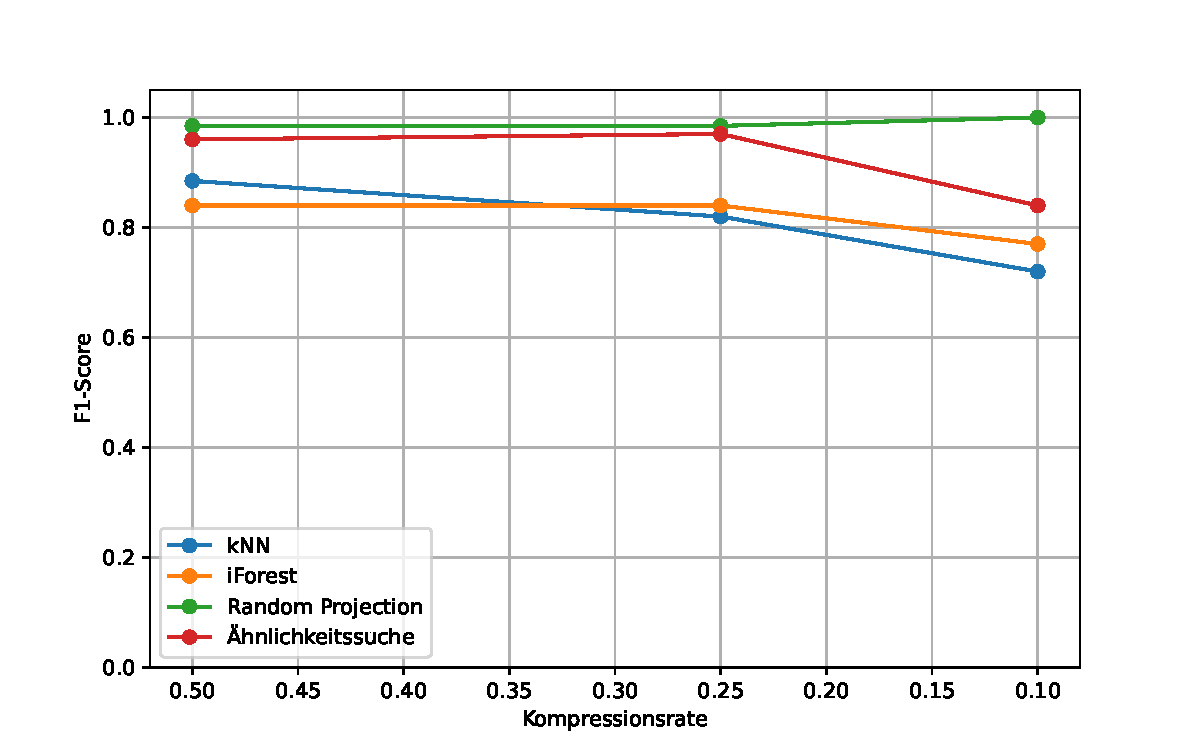
\includegraphics[width=0.49\textwidth]{Graphics/F1LinearWetter.pdf}\label{subfig:f1linwetter}}\hfill
  \subfloat[NVIDIA]{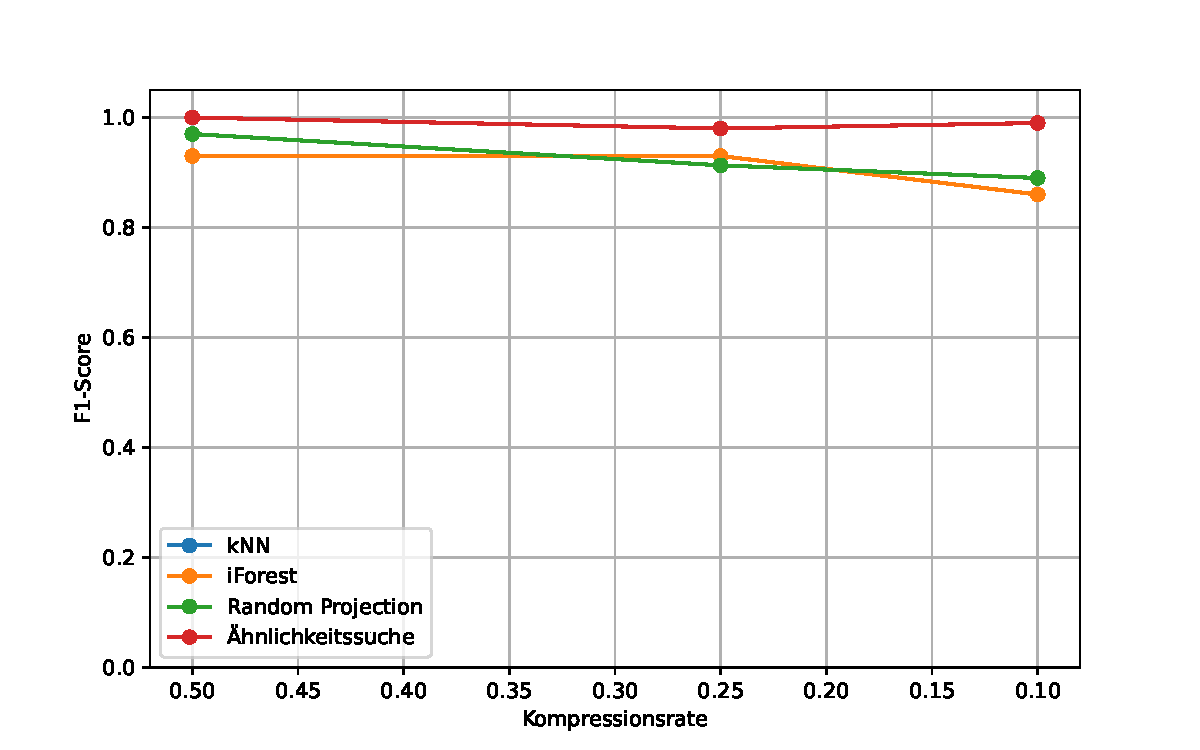
\includegraphics[width=0.49\textwidth]{Graphics/F1LinearNvidia.pdf}\label{subfig:f1linnvidia}}\hfill
  \centering\subfloat[ECG5000]{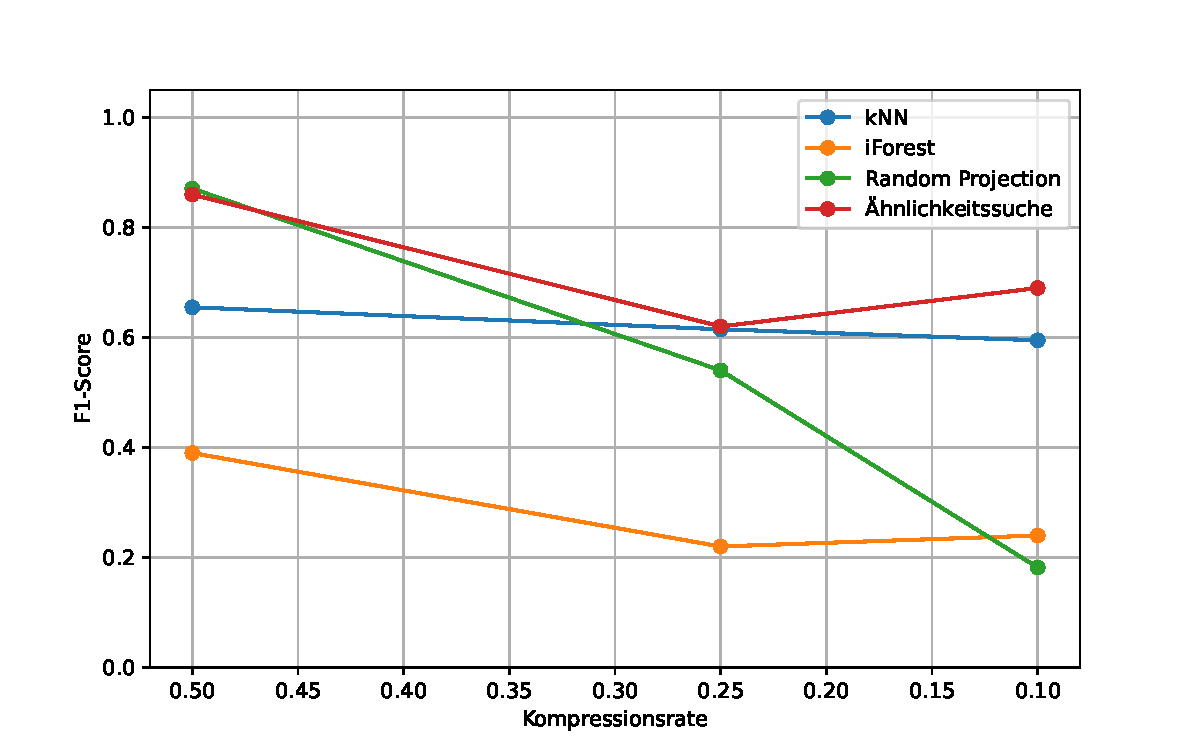
\includegraphics[width=0.49\textwidth]{Graphics/F1LinearECG.pdf}\label{subfig:f1linecg}}
  \caption{F1"=Scores der Analyseverfahren bei linearer Kompression}
  \label{fig:f1LinScores}
\end{figure}

\begin{figure}[bth]
  \subfloat[Wetterdaten]{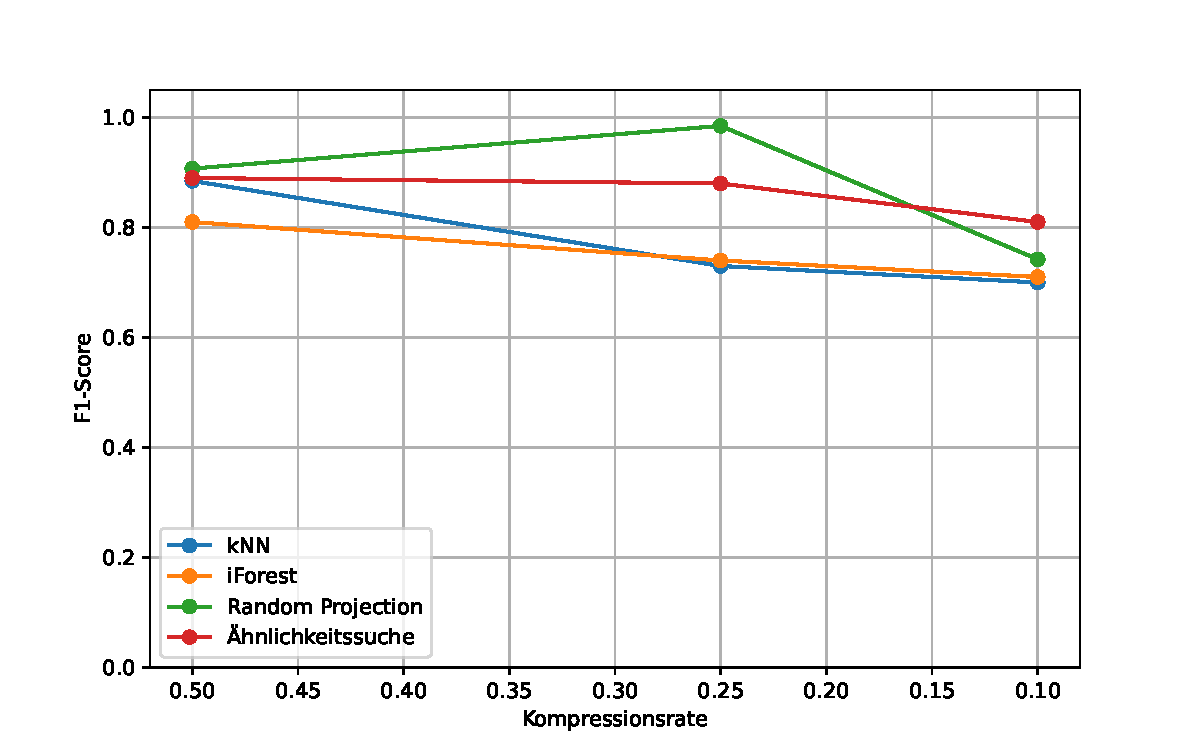
\includegraphics[width=0.49\textwidth]{Graphics/F1PolyWetter.pdf}\label{subfig:f1polwetter}}\hfill
  \subfloat[NVIDIA]{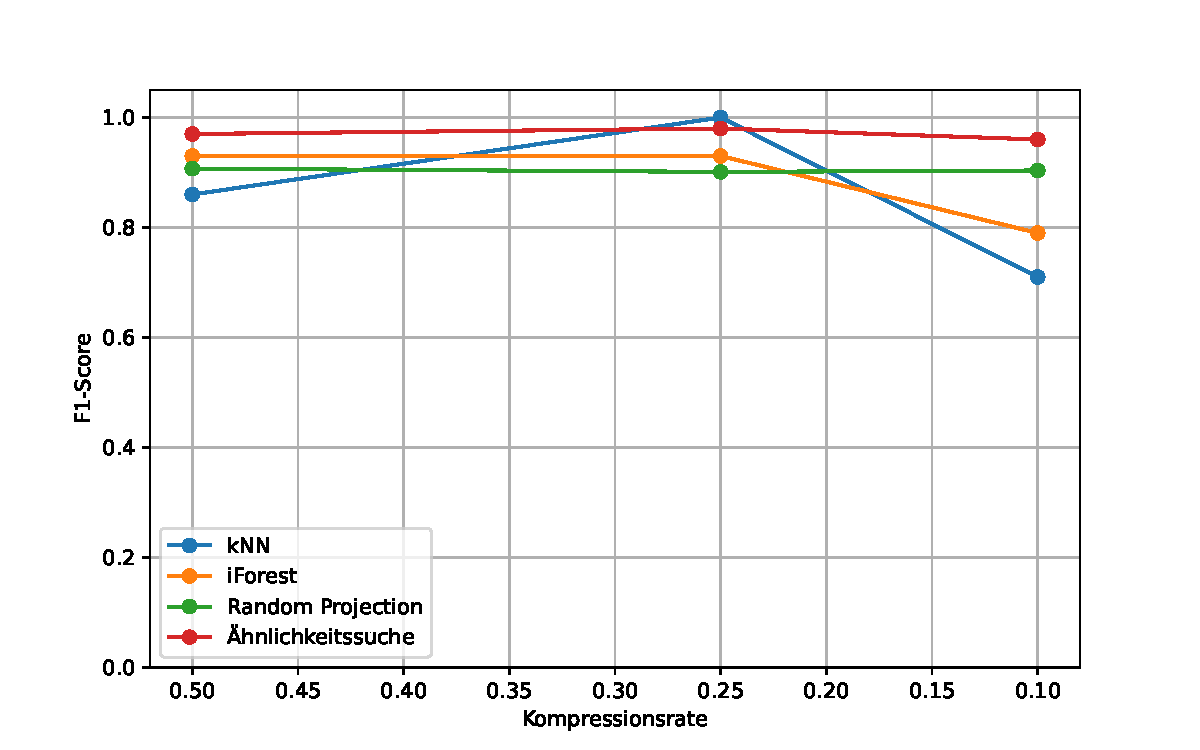
\includegraphics[width=0.49\textwidth]{Graphics/F1PolyNvidia.pdf}\label{subfig:f1polnvidia}}\hfill
  \centering\subfloat[ECG5000]{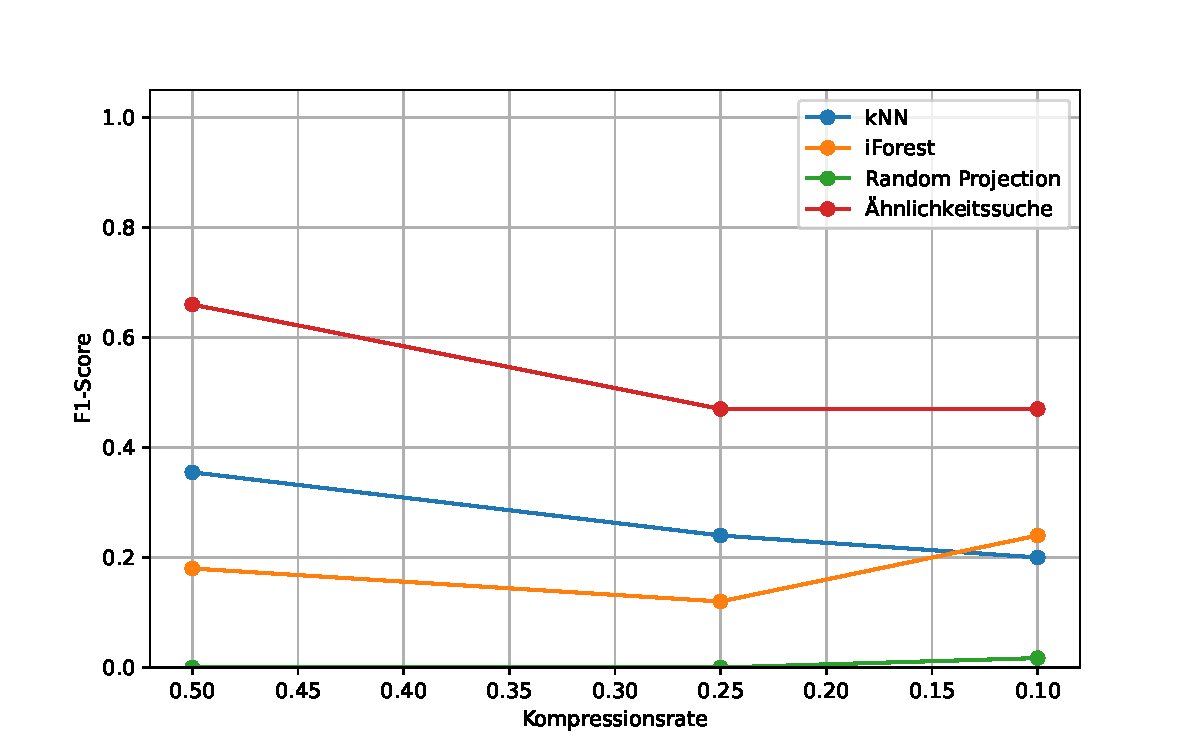
\includegraphics[width=0.49\textwidth]{Graphics/F1PolyECG.pdf}\label{subfig:f1polecg}}
  \caption{F1"=Scores der Analyseverfahren bei polynomieller Kompression}
  \label{fig:f1PolScores}
\end{figure}

\begin{figure}[bth]
  \subfloat[Wetterdaten]{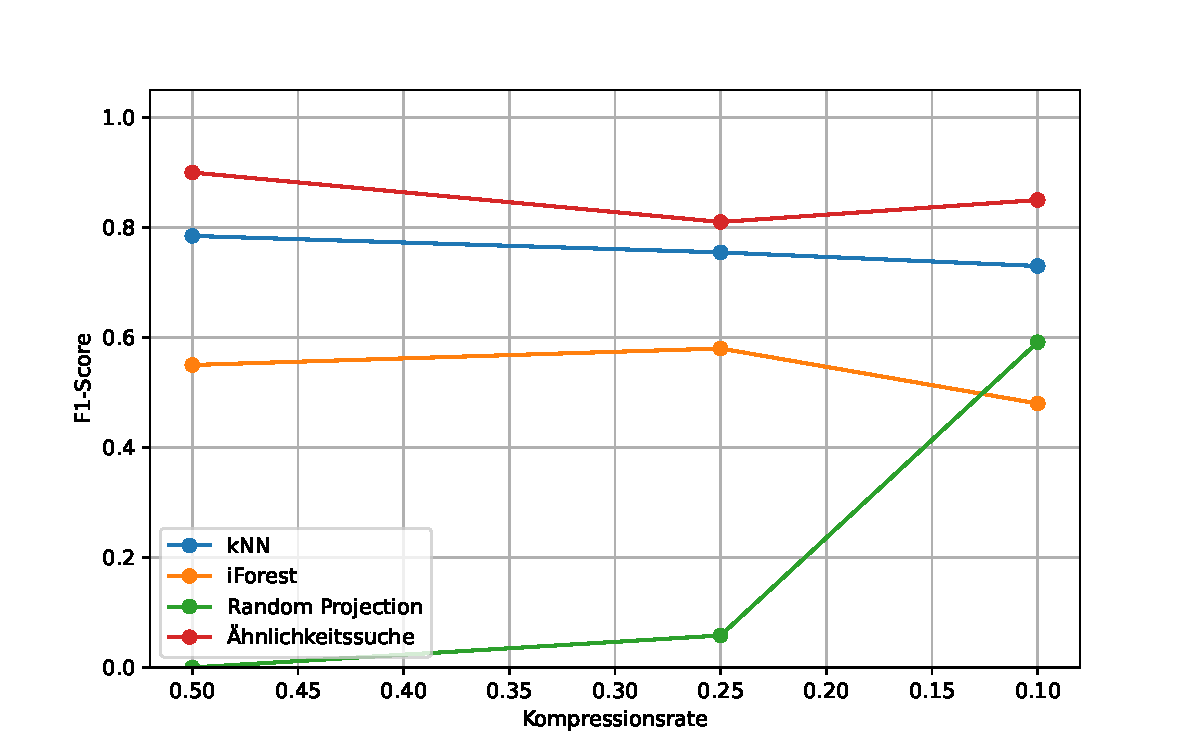
\includegraphics[width=0.49\textwidth]{Graphics/F1FourierWetter.pdf}\label{subfig:f1fourierwetter}}\hfill
  \subfloat[NVIDIA]{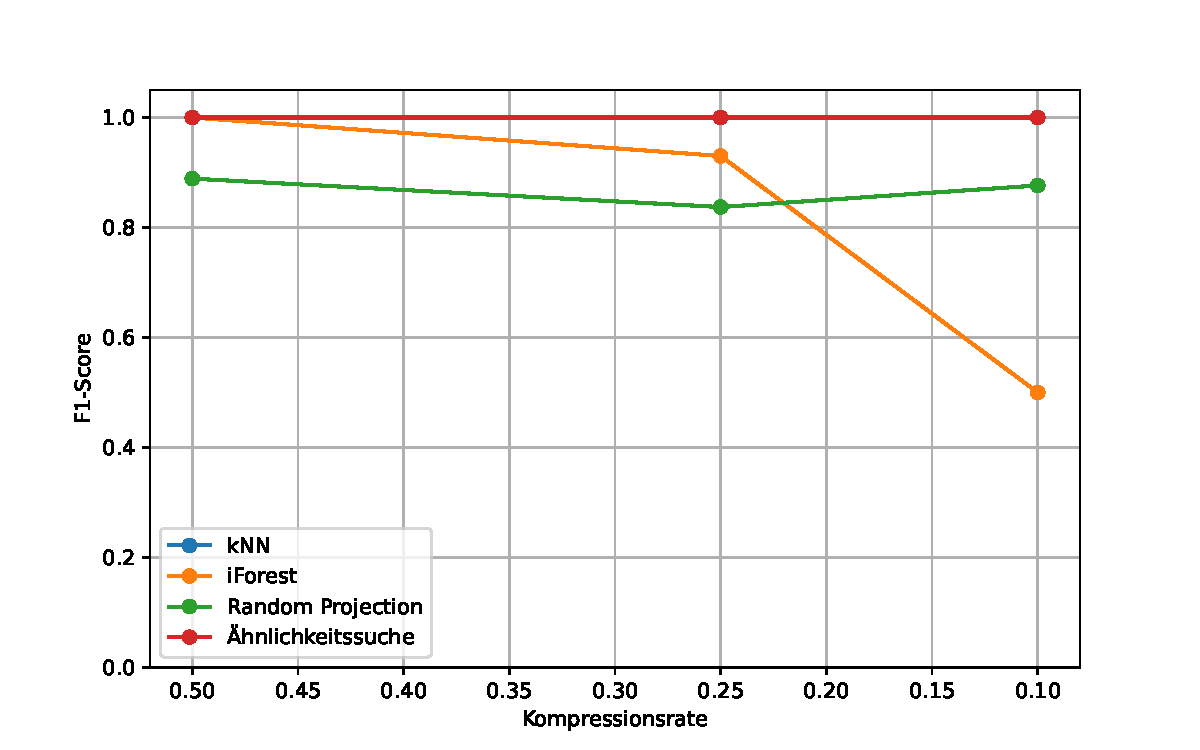
\includegraphics[width=0.49\textwidth]{Graphics/F1FourierNvidia.pdf}\label{subfig:f1fouriernvidia}}\hfill
  \centering\subfloat[ECG5000]{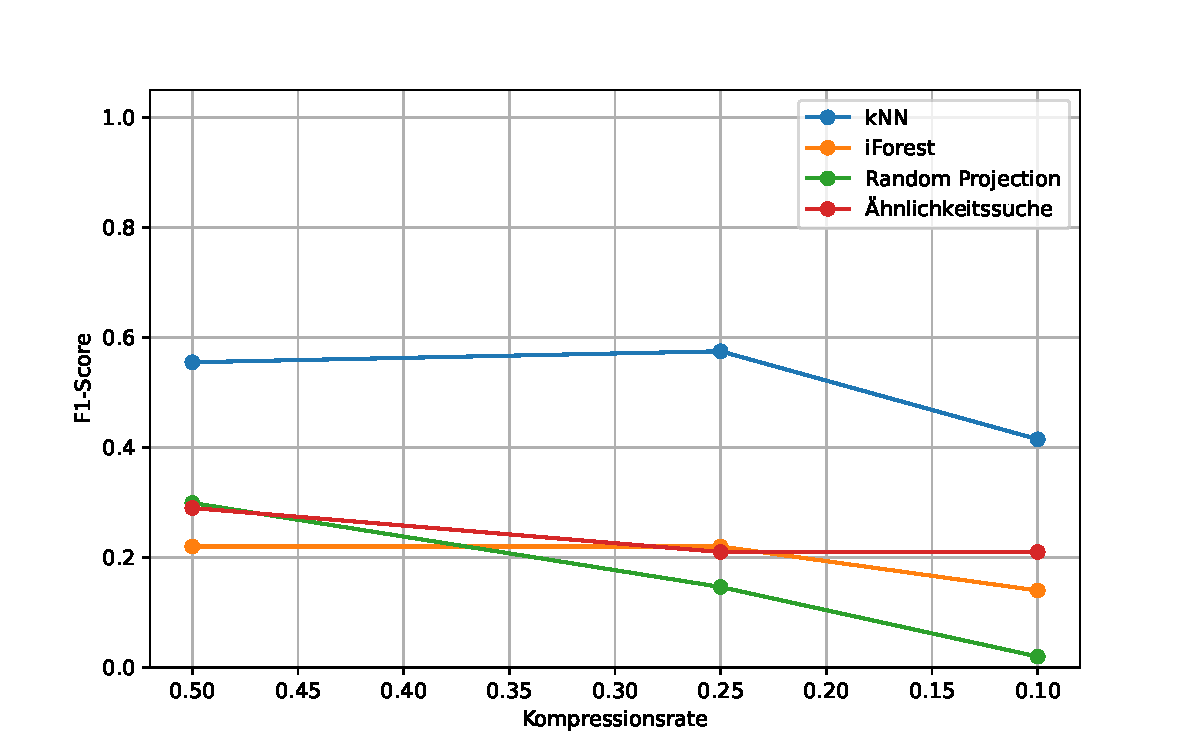
\includegraphics[width=0.49\textwidth]{Graphics/F1FourierECG.pdf}\label{subfig:f1fourierecg}}
  \caption{F1"=Scores der Analyseverfahren bei Fourier"=Kompression}
  \label{fig:f1FourScores}
\end{figure}

\begin{figure}[bth]
  \subfloat[Wetterdaten]{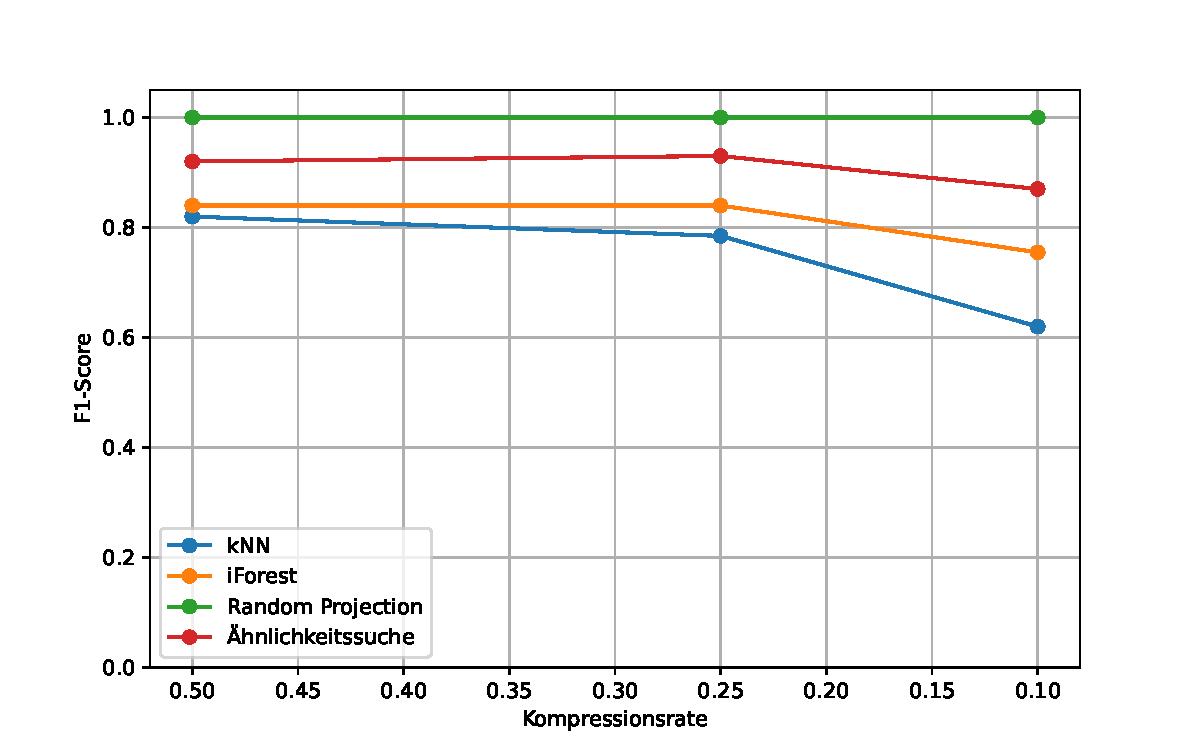
\includegraphics[width=0.49\textwidth]{Graphics/F1WaveletWetter.pdf}\label{subfig:f1waveletwetter}}\hfill
  \subfloat[NVIDIA]{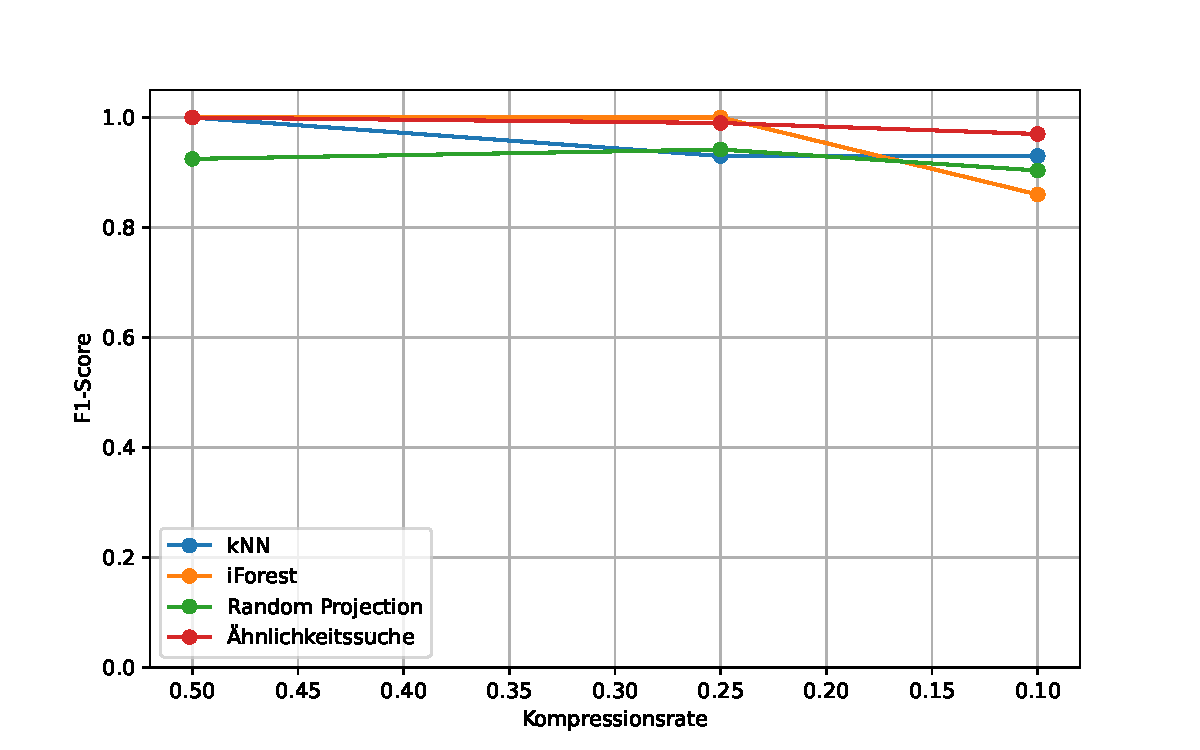
\includegraphics[width=0.49\textwidth]{Graphics/F1WaveletNvidia.pdf}\label{subfig:f1waveletnvidia}}\hfill
  \centering\subfloat[ECG5000]{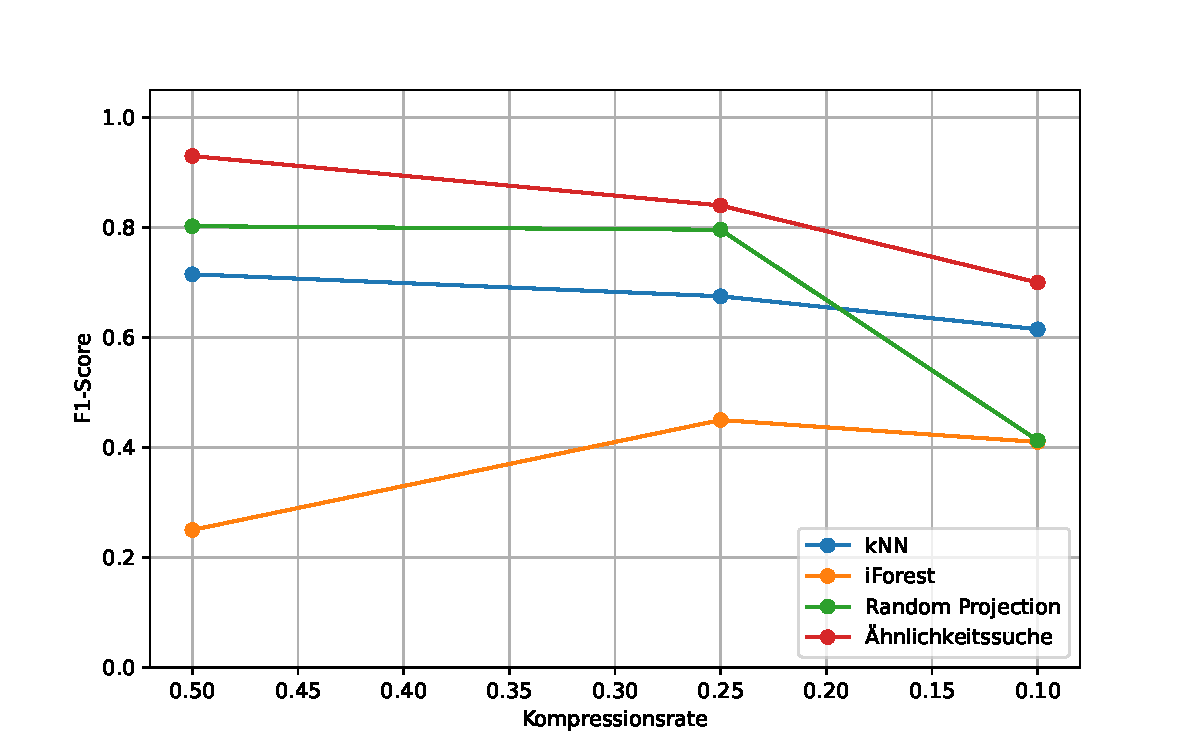
\includegraphics[width=0.49\textwidth]{Graphics/F1WaveletECG.pdf}\label{subfig:f1waveletecg}}
  \caption{F1"=Scores der Analyseverfahren bei Wavelet"=Kompression}
  \label{fig:f1WaveletScores}
\end{figure}

% Lineare Kompression
 \begin{table}[p]
  \centering
  \begin{datatabular}
   \datarowfirst{0,50}{Wetterdaten}{knn} \datarowright{27} {271} {4} {3} {0,90} {0,87}
   \datarownext{iForest} \datarowright{26} {269} {5} {5} {0,84} {0,84}
   \datarownext{Random Projection} \datarowright{38} {266} {1} {0} {1,00} {0,97}
   \datarownext{Ähnlichkeitssuche} \datarowright{96} {201} {4} {4} {0,96} {0,96}
   \datarowfirst{0,50}{NVIDIA-Aktie}{knn} \datarowright{13} {117} {1} {1} {0,93} {0,93}
   \datarownext{iForest} \datarowright{13} {117} {1} {1} {0,93} {0,93}
   \datarownext{Random Projection} \datarowright{34} {96} {1} {1} {0,97} {0,97}
   \datarownext{Ähnlichkeitssuche} \datarowright{100} {32} {0} {0} {1,00} {1,00}
   \datarowfirst{0,50}{ECG5000}{knn} \datarowright{33} {435} {18} {17} {0,66} {0,65}
   \datarownext{iForest} \datarowright{20} {421} {31} {31} {0,39} {0,39}
   \datarownext{Random Projection} \datarowright{58} {428} {2} {15} {0,79} {0,97}
   \datarownext{Ähnlichkeitssuche} \datarowright{86} {389} {14} {14} {0,86} {0,86}
   %
   \datarowfirst{0,25}{Wetterdaten}{knn} \datarowright{25} {269} {6} {5} {0,83} {0,81}
   \datarownext{iForest} \datarowright{26} {269} {5} {5} {0,84} {0,84}
   \datarownext{Random Projection} \datarowright{38} {266} {1} {0} {1,00} {0,97}
   \datarownext{Ähnlichkeitssuche} \datarowright{97} {202} {3} {3} {0,97} {0,97}
   \datarowfirst{0,25}{NVIDIA-Aktie}{knn} \datarowright{13} {117} {1} {1} {0,93} {0,93}
   \datarownext{iForest} \datarowright{13} {117} {1} {1} {0,93} {0,93}
   \datarownext{Random Projection} \datarowright{31} {95} {6} {0} {1,00} {0,84}
   \datarownext{Ähnlichkeitssuche} \datarowright{98} {30} {2} {2} {0,98} {0,98}
   \datarowfirst{0,25}{ECG5000}{knn} \datarowright{31} {433} {20} {19} {0,62} {0,61}
   \datarownext{iForest} \datarowright{11} {412} {40} {40} {0,22} {0,22}
   \datarownext{Random Projection} \datarowright{29} {425} {0} {49} {0,37} {1,00}
   \datarownext{Ähnlichkeitssuche} \datarowright{62} {365} {38} {38} {0,62} {0,62}
   %
  \datarowfirst{0,10}{Wetterdaten}{knn} \datarowright{22} {266} {9} {8} {0,73} {0,71}
   \datarownext{iForest} \datarowright{24} {267} {7} {7} {0,77} {0,77}
   \datarownext{Random Projection} \datarowright{38} {267} {0} {0} {1,00} {1,00}
   \datarownext{Ähnlichkeitssuche} \datarowright{84} {189} {16} {16} {0,84} {0,84}
   \datarowfirst{0,10}{NVIDIA-Aktie}{knn} \datarowright{12} {116} {2} {2} {0,86} {0,86}
   \datarownext{iForest} \datarowright{12} {116} {2} {2} {0,86} {0,86}
   \datarownext{Random Projection} \datarowright{31} {93} {4} {4} {0,89} {0,89}
   \datarownext{Ähnlichkeitssuche} \datarowright{99} {31} {1} {1} {0,99} {0,99}
   \datarowfirst{0,10}{ECG5000}{knn} \datarowright{30} {432} {21} {20} {0,60} {0,59}
   \datarownext{iForest} \datarowright{12} {413} {39} {39} {0,24} {0,24}
   \datarownext{Random Projection} \datarowright{8} {419} {0} {76} {0,10} {1,00}
   \datarownext{Ähnlichkeitssuche} \datarowright{69} {372} {31} {31} {0,69} {0,69}
  \end{datatabular}
  \caption{Kompressionsverfahren: Linear}\label{tab:datakomplin}
 \end{table}

 % Polynomielle Kompression
 \begin{table}[p]
  \centering
  \begin{datatabular}
   \datarowfirst{0,50}{Wetterdaten}{knn} \datarowright{27} {271} {4} {3} {0,90} {0,87}
   \datarownext{iForest} \datarowright{25} {268} {6} {6} {0,81} {0,81}
   \datarownext{Random Projection} \datarowright{38} {259} {8} {0} {1,00} {0,83}
   \datarownext{Ähnlichkeitssuche} \datarowright{89} {194} {11} {11} {0,89} {0,89}
   \datarowfirst{0,50}{NVIDIA-Aktie}{knn} \datarowright{12} {116} {2} {2} {0,86} {0,86}
   \datarownext{iForest} \datarowright{13} {117} {1} {1} {0,93} {0,93}
   \datarownext{Random Projection} \datarowright{35} {90} {7} {0} {1,00} {0,83}
   \datarownext{Ähnlichkeitssuche} \datarowright{97} {29} {3} {3} {0,97} {0,97}
   \datarowfirst{0,50}{ECG5000}{knn} \datarowright{18} {420} {33} {32} {0,36} {0,35}
   \datarownext{iForest} \datarowright{9} {410} {42} {42} {0,18} {0,18}
   \datarownext{Random Projection} \datarowright{0} {428} {2} {73} {0,00} {0,00}
   \datarownext{Ähnlichkeitssuche} \datarowright{66} {369} {34} {34} {0,66} {0,66}
   %
   \datarowfirst{0,25}{Wetterdaten}{knn} \datarowright{22} {267} {8} {8} {0,73} {0,73}
   \datarownext{iForest} \datarowright{23} {266} {8} {8} {0,74} {0,74}
   \datarownext{Random Projection} \datarowright{37} {267} {0} {1} {0,97} {1,00}
   \datarownext{Ähnlichkeitssuche} \datarowright{88} {193} {12} {12} {0,88} {0,88}
   \datarowfirst{0,25}{NVIDIA-Aktie}{knn} \datarowright{14} {118} {0} {0} {1,00} {1,00}
   \datarownext{iForest} \datarowright{13} {117} {1} {1} {0,93} {0,93}
   \datarownext{Random Projection} \datarowright{31} {94} {7} {0} {1,00} {0,82}
   \datarownext{Ähnlichkeitssuche} \datarowright{98} {30} {2} {2} {0,98} {0,98}
   \datarowfirst{0,25}{ECG5000}{knn} \datarowright{12} {414} {39} {38} {0,24} {0,24}
   \datarownext{iForest} \datarowright{6} {407} {45} {45} {0,12} {0,12}
   \datarownext{Random Projection} \datarowright{0} {423} {2} {78} {0,00} {0,00}
   \datarownext{Ähnlichkeitssuche} \datarowright{47} {350} {53} {53} {0,47} {0,47}
   %
   \datarowfirst{0,10}{Wetterdaten}{knn} \datarowright{21} {266} {9} {9} {0,70} {0,70}
   \datarownext{iForest} \datarowright{22} {265} {9} {9} {0,71} {0,71}
   \datarownext{Random Projection} \datarowright{38} {241} {26} {0} {1,00} {0,59}
   \datarownext{Ähnlichkeitssuche} \datarowright{81} {186} {19} {19} {0,81} {0,81}
   \datarowfirst{0,10}{NVIDIA-Aktie}{knn} \datarowright{10} {114} {4} {4} {0,71} {0,71}
   \datarownext{iForest} \datarowright{11} {115} {3} {3} {0,79} {0,79}
   \datarownext{Random Projection} \datarowright{33} {92} {5} {2} {0,94} {0,87}
   \datarownext{Ähnlichkeitssuche} \datarowright{96} {28} {4} {4} {0,96} {0,96}
   \datarowfirst{0,10}{ECG5000}{knn} \datarowright{10} {412} {41} {40} {0,20} {0,20}
   \datarownext{iForest} \datarowright{12} {413} {39} {39} {0,24} {0,24}
   \datarownext{Random Projection} \datarowright{1} {404} {15} {83} {0,01} {0,06}
   \datarownext{Ähnlichkeitssuche} \datarowright{47} {350} {53} {53} {0,47} {0,47}
  \end{datatabular}
  \caption{Kompressionsverfahren: Polynomiell}\label{tab:datakomppol}
 \end{table}

 % Fourier Kompression
\begin{table}[p]
  \centering
  \begin{datatabular}
   \datarowfirst{0,50}{Wetterdaten}{knn} \datarowright{24} {268} {7} {6} {0,80} {0,77}
   \datarownext{iForest} \datarowright{17} {260} {14} {14} {0,55} {0,55}
   \datarownext{Random Projection} \datarowright{0} {267} {0} {38} {0,00} {0,00}
   \datarownext{Ähnlichkeitssuche} \datarowright{90} {195} {10} {10} {0,90} {0,90}
   \datarowfirst{0,50}{NVIDIA-Aktie}{knn} \datarowright{14} {118} {0} {0} {1,00} {1,00}
   \datarownext{iForest} \datarowright{14} {118} {0} {0} {1,00} {1,00}
   \datarownext{Random Projection} \datarowright{35} {88} {9} {0} {1,00} {0,80}
   \datarownext{Ähnlichkeitssuche} \datarowright{100} {32} {0} {0} {1,00} {1,00}
   \datarowfirst{0,50}{ECG5000}{knn} \datarowright{28} {430} {23} {22} {0,56} {0,55}
   \datarownext{iForest} \datarowright{11} {412} {40} {40} {0,22} {0,22}
   \datarownext{Random Projection} \datarowright{15} {416} {14} {58} {0,21} {0,52}
   \datarownext{Ähnlichkeitssuche} \datarowright{29} {332} {71} {71} {0,29} {0,29}
   %
   \datarowfirst{0,25}{Wetterdaten}{knn} \datarowright{23} {267} {8} {7} {0,77} {0,74}
   \datarownext{iForest} \datarowright{18} {261} {13} {13} {0,58} {0,58}
   \datarownext{Random Projection} \datarowright{1} {267} {0} {37} {0,03} {1,00}
   \datarownext{Ähnlichkeitssuche} \datarowright{81} {186} {19} {19} {0,81} {0,81}
   \datarowfirst{0,25}{NVIDIA-Aktie}{knn} \datarowright{14} {118} {0} {0} {1,00} {1,00}
   \datarownext{iForest} \datarowright{13} {117} {1} {1} {0,93} {0,93}
   \datarownext{Random Projection} \datarowright{31} {89} {12} {0} {1,00} {0,72}
   \datarownext{Ähnlichkeitssuche} \datarowright{100} {32} {0} {0} {1,00} {1,00}
   \datarowfirst{0,25}{ECG5000}{knn} \datarowright{29} {431} {22} {21} {0,58} {0,57}
   \datarownext{iForest} \datarowright{11} {412} {40} {40} {0,22} {0,22}
   \datarownext{Random Projection} \datarowright{6} {424} {1} {72} {0,08} {0,86}
   \datarownext{Ähnlichkeitssuche} \datarowright{21} {324} {79} {79} {0,21} {0,21}
   %
   \datarowfirst{0,10}{Wetterdaten}{knn} \datarowright{22} {267} {8} {8} {0,73} {0,73}
   \datarownext{iForest} \datarowright{15} {258} {16} {16} {0,48} {0,48}
   \datarownext{Random Projection} \datarowright{16} {267} {0} {22} {0,42} {1,00}
   \datarownext{Ähnlichkeitssuche} \datarowright{85} {190} {15} {15} {0,85} {0,85}
   \datarowfirst{0,10}{NVIDIA-Aktie}{knn} \datarowright{14} {118} {0} {0} {1,00} {1,00}
   \datarownext{iForest} \datarowright{7} {111} {7} {7} {0,50} {0,50}
   \datarownext{Random Projection} \datarowright{35} {87} {10} {0} {1,00} {0,78}
   \datarownext{Ähnlichkeitssuche} \datarowright{100} {32} {0} {0} {1,00} {1,00}
   \datarowfirst{0,10}{ECG5000}{knn} \datarowright{21} {423} {30} {29} {0,42} {0,41}
   \datarownext{iForest} \datarowright{7} {408} {44} {44} {0,14} {0,14}
   \datarownext{Random Projection} \datarowright{1} {419} {0} {83} {0,01} {1,00}
   \datarownext{Ähnlichkeitssuche} \datarowright{21} {324} {79} {79} {0,21} {0,21}
  \end{datatabular}
  \caption{Kompressionsverfahren: Fourier}\label{tab:datakompfour}
 \end{table}

 % Wavelet Kompression
\begin{table}[p]
  \centering
  \begin{datatabular}
   \datarowfirst{0,50}{Wetterdaten}{knn} \datarowright{25} {269} {6} {5} {0,83} {0,81}
   \datarownext{iForest} \datarowright{26} {269} {5} {5} {0,84} {0,84}
   \datarownext{Random Projection} \datarowright{38} {267} {0} {0} {1,00} {1,00}
   \datarownext{Ähnlichkeitssuche} \datarowright{92} {197} {8} {8} {0,92} {0,92}
   \datarowfirst{0,50}{NVIDIA-Aktie}{knn} \datarowright{14} {118} {0} {0} {1,00} {1,00}
   \datarownext{iForest} \datarowright{14} {118} {0} {0} {1,00} {1,00}
   \datarownext{Random Projection} \datarowright{32} {95} {2} {3} {0,91} {0,94}
   \datarownext{Ähnlichkeitssuche} \datarowright{100} {32} {0} {0} {1,00} {1,00}
   \datarowfirst{0,50}{ECG5000}{knn} \datarowright{36} {438} {15} {14} {0,72} {0,71}
   \datarownext{iForest} \datarowright{13} {414} {38} {38} {0,25} {0,25}
   \datarownext{Random Projection} \datarowright{49} {430} {0} {24} {0,67} {1,00}
   \datarownext{Ähnlichkeitssuche} \datarowright{93} {396} {7} {7} {0,93} {0,93}
   %
   \datarowfirst{0,25}{Wetterdaten}{knn} \datarowright{24} {268} {7} {6} {0,80} {0,77}
   \datarownext{iForest} \datarowright{26} {269} {5} {5} {0,84} {0,84}
   \datarownext{Random Projection} \datarowright{38} {267} {0} {0} {1,00} {1,00}
   \datarownext{Ähnlichkeitssuche} \datarowright{93} {198} {7} {7} {0,93} {0,93}
   \datarowfirst{0,25}{NVIDIA-Aktie}{knn} \datarowright{13} {117} {1} {1} {0,93} {0,93}
   \datarownext{iForest} \datarowright{14} {118} {0} {0} {1,00} {1,00}
   \datarownext{Random Projection} \datarowright{31} {97} {4} {0} {1,00} {0,89}
   \datarownext{Ähnlichkeitssuche} \datarowright{99} {31} {1} {1} {0,99} {0,99}
   \datarowfirst{0,25}{ECG5000}{knn} \datarowright{34} {436} {17} {16} {0,68} {0,67}
   \datarownext{iForest} \datarowright{23} {424} {28} {28} {0,45} {0,45}
   \datarownext{Random Projection} \datarowright{52} {424} {1} {26} {0,67} {0,98}
   \datarownext{Ähnlichkeitssuche} \datarowright{84} {387} {16} {16} {0,84} {0,84}
   %
   \datarowfirst{0,10}{Wetterdaten}{knn} \datarowright{19} {263} {12} {11} {0,63} {0,61}
   \datarownext{iForest} \datarowright{23} {267} {7} {8} {0,74} {0,77}
   \datarownext{Random Projection} \datarowright{38} {267} {0} {0} {1,00} {1,00}
   \datarownext{Ähnlichkeitssuche} \datarowright{87} {192} {13} {13} {0,87} {0,87}
   \datarowfirst{0,10}{NVIDIA-Aktie}{knn} \datarowright{13} {117} {1} {1} {0,93} {0,93}
   \datarownext{iForest} \datarowright{12} {116} {2} {2} {0,86} {0,86}
   \datarownext{Random Projection} \datarowright{33} {92} {5} {2} {0,94} {0,87}
   \datarownext{Ähnlichkeitssuche} \datarowright{97} {29} {3} {3} {0,97} {0,97}
   \datarowfirst{0,10}{ECG5000}{knn} \datarowright{31} {433} {20} {19} {0,62} {0,61}
   \datarownext{iForest} \datarowright{21} {422} {30} {30} {0,41} {0,41}
   \datarownext{Random Projection} \datarowright{22} {419} {0} {62} {0,26} {1,00}
   \datarownext{Ähnlichkeitssuche} \datarowright{70} {373} {30} {30} {0,70} {0,70}
  \end{datatabular}
  \caption{Kompressionsverfahren: Wavelet}\label{tab:datakompwav}
 \end{table}